\section{Benutzeroberfläche}
%[TODO: remove this link] https://tex.stackexchange.com/questions/442077/is-it-possible-to-use-svg-images-with-overleaf

%[TODO: Arrange the images correctly, probably see here https://de.overleaf.com/learn/latex/Inserting_Images]
\subsection{Bilder des Entwurfs}
\begin{figure}[h]
    \centering

        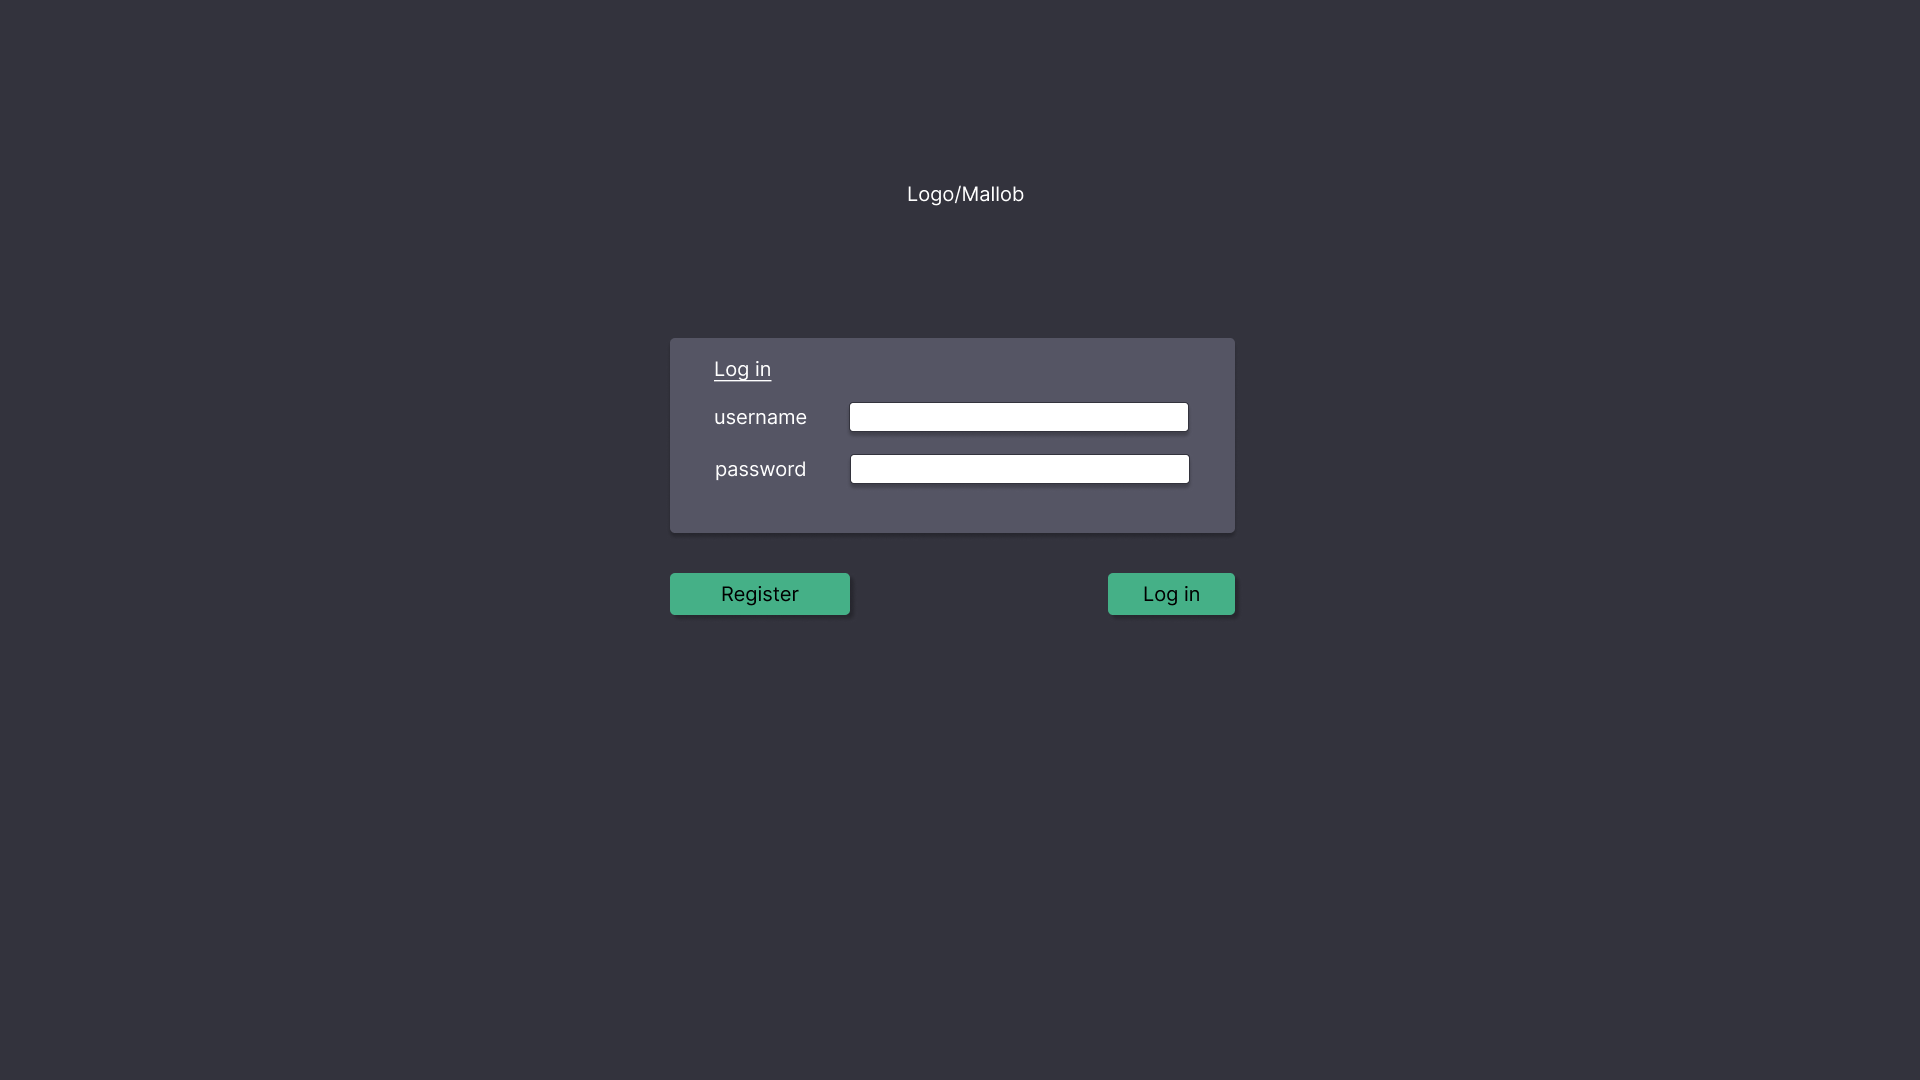
\includegraphics[width=\textwidth]{images-interface/Loginv1.png}
        \caption{Anmelde-Maske}
        \label{fig:login}
   
        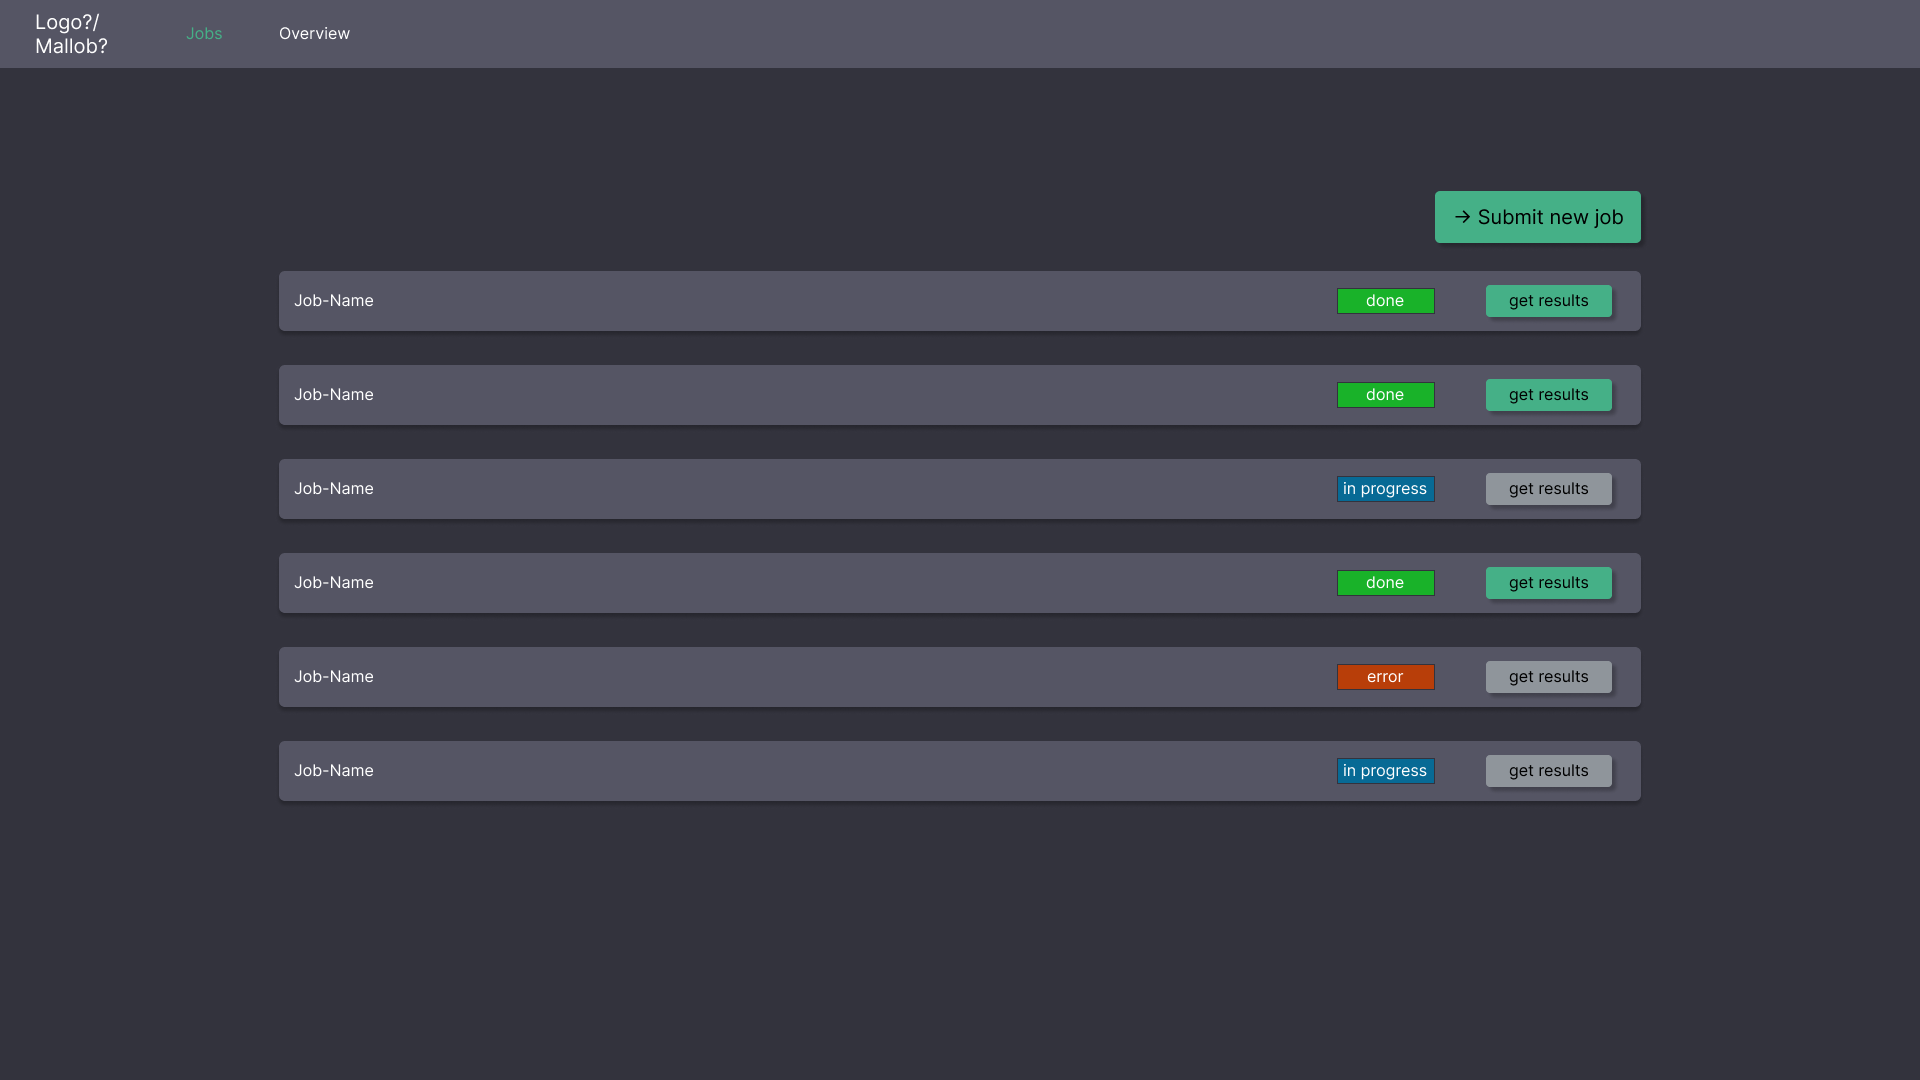
\includegraphics[width=\textwidth]{images-interface/Job-Viewv1.png}
        \caption{Auftrags-Übersicht}
        \label{fig:viewjobs}
  
\end{figure}


\begin{figure}[h]
    \centering
    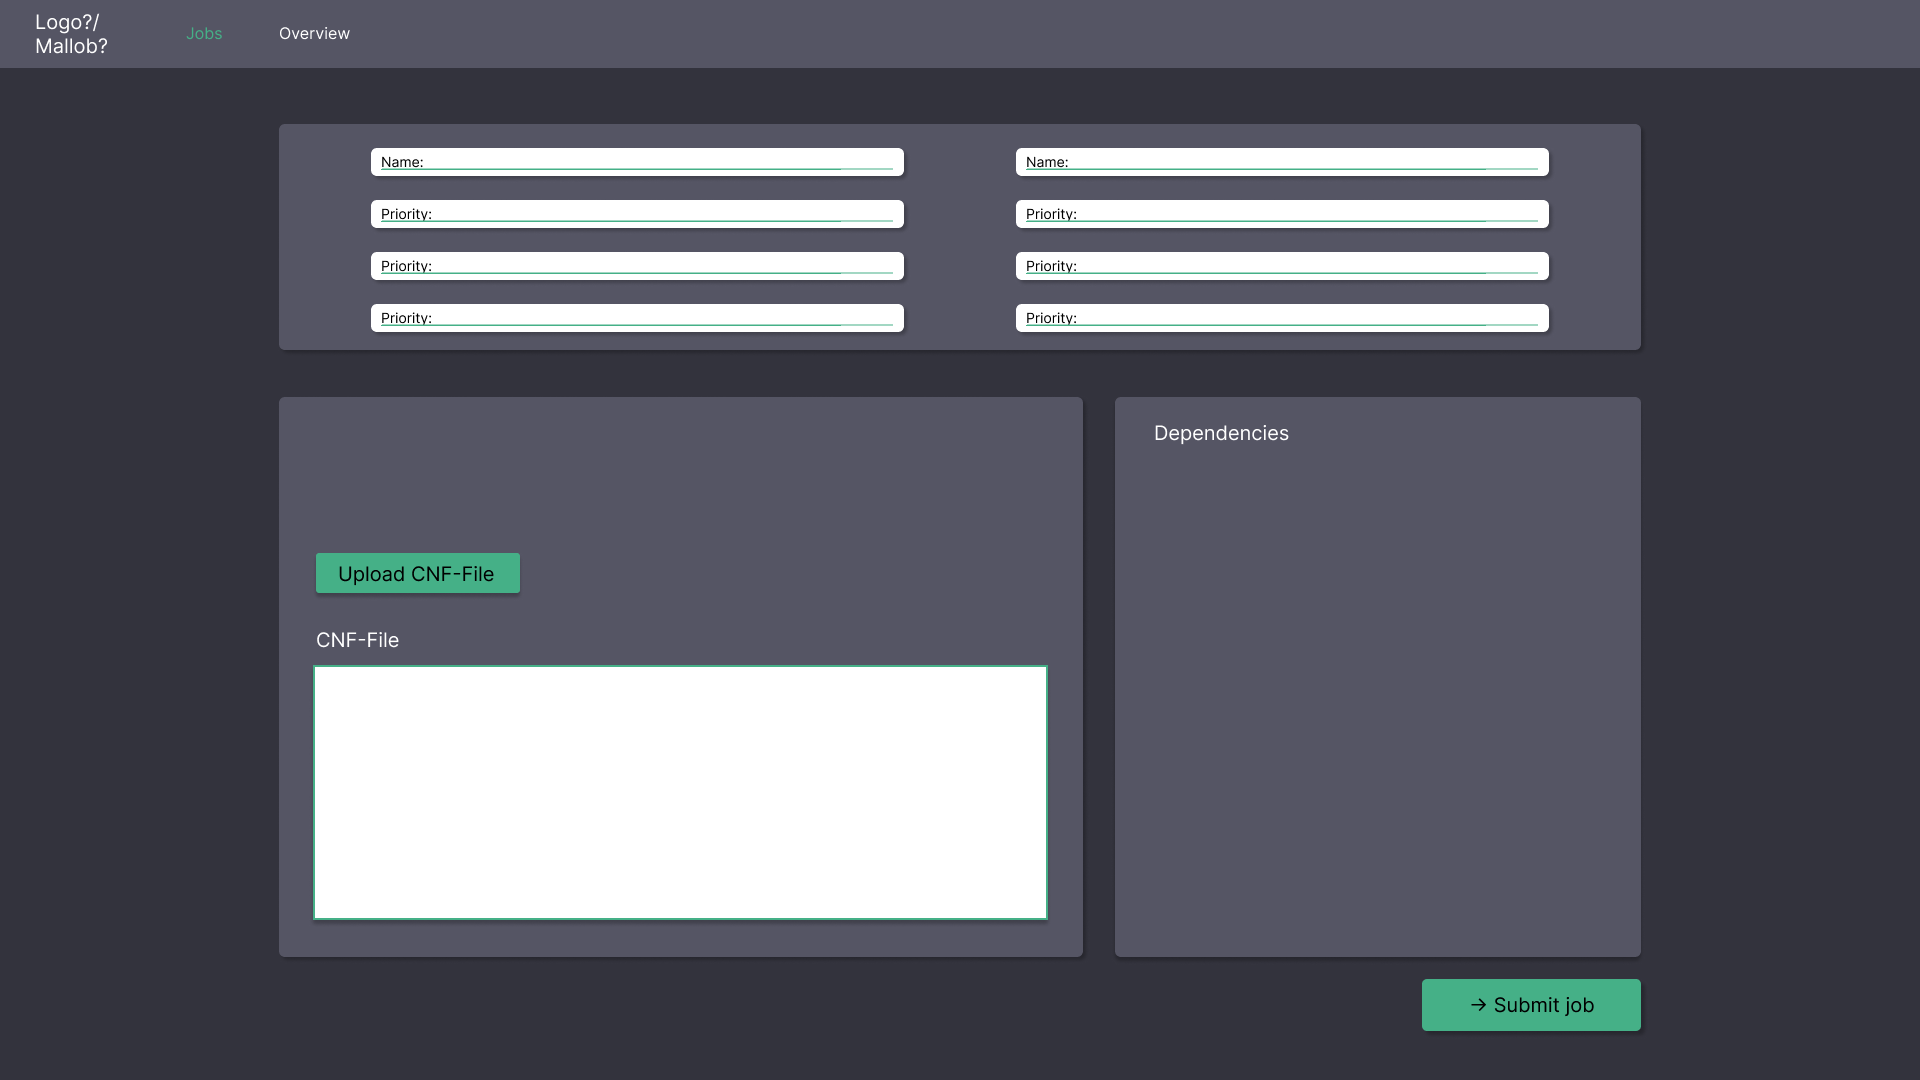
\includegraphics[width=\textwidth]{images-interface/Submit-Filev1.png}
    \caption{Maske zum Hinzufügen neuer Aufträge}
    \label{fig:addjobs}
     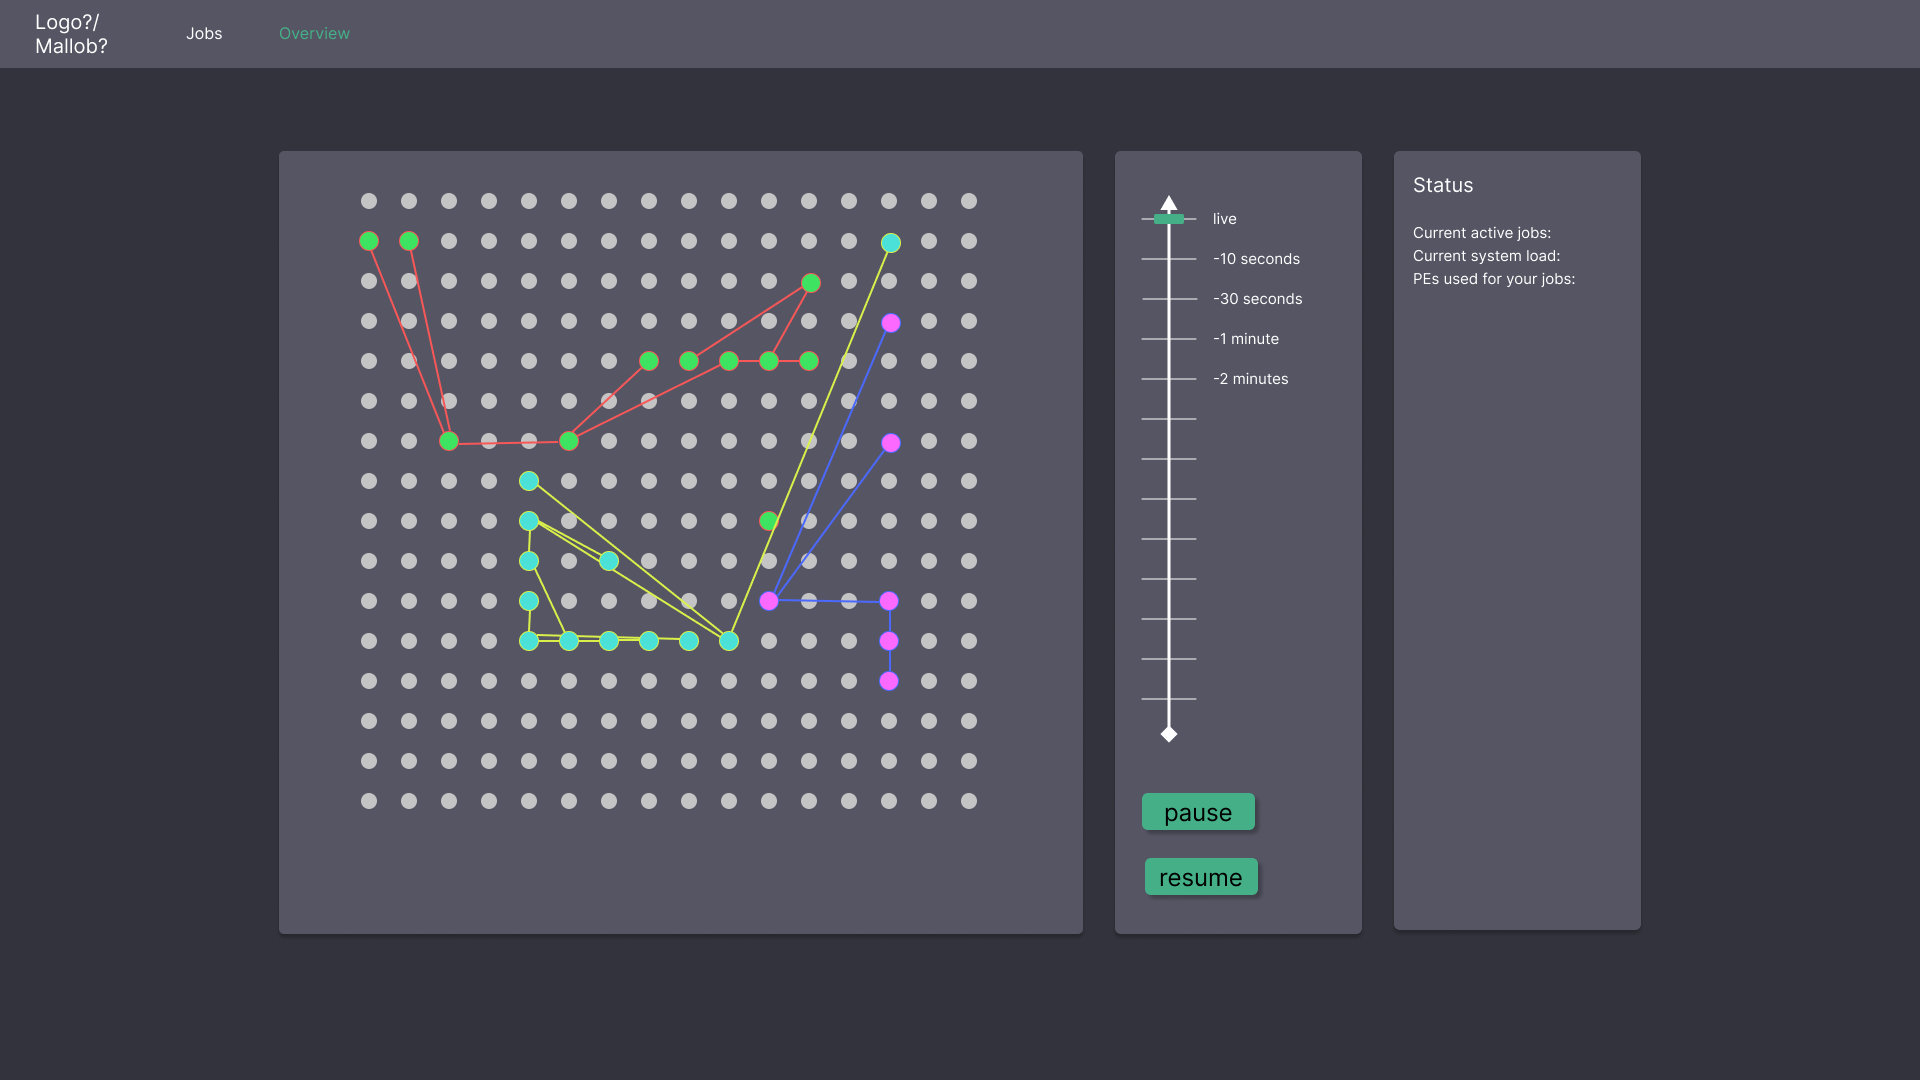
\includegraphics[width=\textwidth]{images-interface/overviewv1.png}
    \caption{Visualisierung des Systems}
    \label{fig:visualsn}
\end{figure}


\subsection{Funktionen}
\begin{itemize}
    \item /B010/ Es sind zwei Sichten zu unterscheiden: die des Admins, die des Benutzers. 
    \item /B020/ Benutzer können Funktionen F10, F20, F30 jederzeit nach dem Einloggen aufrufen.
    \item /B030/ Jeder Benutzer fängt auf der Login/Register-Seite an.
    \item /B040/ Sobald der Benutzer eingeloggt wird, sieht er die Startseite.
    \item /B050/ Jeder Nutzer kann seine Jobs anhand der Aufwand auf das Kern unterscheiden (z.B Farbe, Größe usw.)
    \item /B060/ Admins können alle Funktionen, die die Benutzer können.
    \item /B070/ Unterschiedliche Benutzer und ihre Befugnisse sollen entsprechend behandelt werden (nicht-funktionale Anforderung?).
    \item /B080/ Die Bedienungsoberfläche ist auf Mausbedienung auszulegen; eine Bedienung ohne Maus muss aber auch möglich sein. ([TODO] Bediengung ohne Maus auf jeden Fall wunschkriterium oder vlt sogar gar nicth, auf jeden Fall mal fragen, hört sich kompliziert und nicht wirklich notwendig an)
\end{itemize}